\documentclass[a4paper,12pt]{article}
\usepackage[T1]{fontenc}
\usepackage[utf8]{inputenc}
\usepackage{lmodern}
\usepackage{amsmath}
\usepackage{amsfonts}
\usepackage{amssymb}
\usepackage{amsthm}
\usepackage{graphicx}
\usepackage{color}
\usepackage{xcolor}
\usepackage{url}
\usepackage{theorem}
\usepackage{textcomp}
\usepackage{listings}
\usepackage{hyperref}
\usepackage{parskip}

\title{Počítačové architektury číslicových strojů}
\author{Vojtech Vasek}

\begin{document}
\begin{center}
    \huge{\underline{\textbf{Počítačové architektury číslicových strojů}}}
\end{center}
\begin{itemize}
    \item{rozlišujeme dvě základní architektury}
    \item{moderní procesory spojují obě architektury; uvnitř procesoru Harvardská; zvenku von Neumannova}
\end{itemize}

\section{Von Neumannova architektura}
    \begin{itemize}
        \item{označuje jednoduché schéma počítače používající jednu sběrnici}
        \item{jméno architektura získala po přednášce matematika Johna von Neumanna}
        \item{architektura popisuje počítač se společnou pamětí pro instrukce i data tudíž zpracování je sekvenční}
        \item{procesor se skládá z řídící jednotky a výkonné ALU; řídící zpracovává instrukce v paměti; výkonná jednotka následně operuje s daty podle instrukcí. vstup a výstup dat mají na starosti vstupní a výstupní jednotky}
        \item{rychlost zpracování instrukcí je dnes výrazně rychlejší než rychlost komunikace s pamětí. tuto nevýhodu částečně řeší mezipaměť (potřebná data a instrukce se do ní načítají rychleji, než jsou při zpracování potřeba)}
        \item{dnes je používána např. v kalkulačkách}
    \end{itemize}
    \begin{figure}[htp]
        \centering
        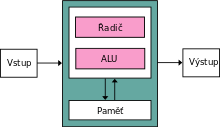
\includegraphics[width=8cm]{TVP_1_10_23@3.png}
    \end{figure}

\section{Harvardská architektura}
    \begin{itemize}
        \item{odděluje fyzický paměť programu a jejich spojovací obvody}
        \item{název pochází z prvního počítače využívající tuto architekturu Harvard Mark I; instrukce byly uloženy na děrované pásce a data na elektromechanických deskách}
        \item{CPU může současně číst instrukci z programové paměti a přistupovat do paměti dat}
        \item{používá se ve specializovaných procesorech, obvykle v audio/video technice}
    \end{itemize}
    \subsection{Paměť}
        \begin{itemize}
            \item{není třeba mít paměť stejných parametrů a vlastností}
            \item{dvojí paměť umožňuje paralelní přístup k oběma pamětím => vyšší rychlost zpracování}
            \item{umístění programu do ROM paměti může zvýšit bezpečnost systému (program nelze modifikovat)}
        \end{itemize}
    \subsection{Rychlost}
        \begin{itemize}
            \item{rychlost procesorů se několikanásobně zvětšila o proti rychlosti hlavní paměti → tendence zredukovat počet přístupů do hl. paměti.}
            \item{za vyšší cenu procesor může být mnohem rychlejší}
            \item{paměť cache (vyrovnávací) je velmi rychlá; je jí méně než hl. paměti; velikost cache je jeden z hlavních aspektů určování rychlosti procesoru}
        \end{itemize}

\section{Sekvenční obvody}
    \begin{itemize}
        \item{nezávisí na okamžité hodnotě vstupních signálů ale i na pořadí minulých vstupů}
        \item{jsou schopny uchovávat stav (obsahují paměť); je potřeba sledovat kromě vstupních proměnných i vnitřní proměnné}
        \item{dělíme na synchronní a asynchronní}
            \item[-] u asynchronních se změna vstupu promítne ihned do stavu obvodu
            \item[-] u synchronních je zaveden synchronizační signál (hodiny); změna vstupu se promítne do obvodu až při pulzu hodinového signálu
        \item{paměťová část je tvořena kombinačním obvodem - bistabilní klopný obvod; jeho úkol je uchovat informaci na vstupu i poté, co informace na vstupu již není}
    \end{itemize}

\section{Kombinační obvody}
    \begin{itemize}
        \item{výstup závisí na okamžité kombinaci vstupů}
        \item{nemají žádnou paměť}
        \item{závislost výstupní funkce je popsána pravdivostní tabulkou nebo pomocí logických výrazů}
        \item{pro realizaci je možné využít}
            \item[\ -]{pevné paměti}
            
            %\SubItem základní logické členy %(NAND; AND, NOR, OR, atd.)
    \end{itemize}

\end{document}
